\thispagestyle{timhieukhoahocnone}
\pagestyle{timhieukhoahoc}
\everymath{\color{timhieukhoahoc}}
\blfootnote{$^1$\text{\color{timhieukhoahoc}Nguồn: Tia Sáng https://tiasang.com.vn/khoa-hoc-cong-nghe/nobel-y-hoc-2022-ky-cuoi-tai-sao-loai-nguoi-song-sot/.}}
\graphicspath{{../timhieukhoahoc/pic/}}
\begingroup
\AddToShipoutPicture*{\put(0,616){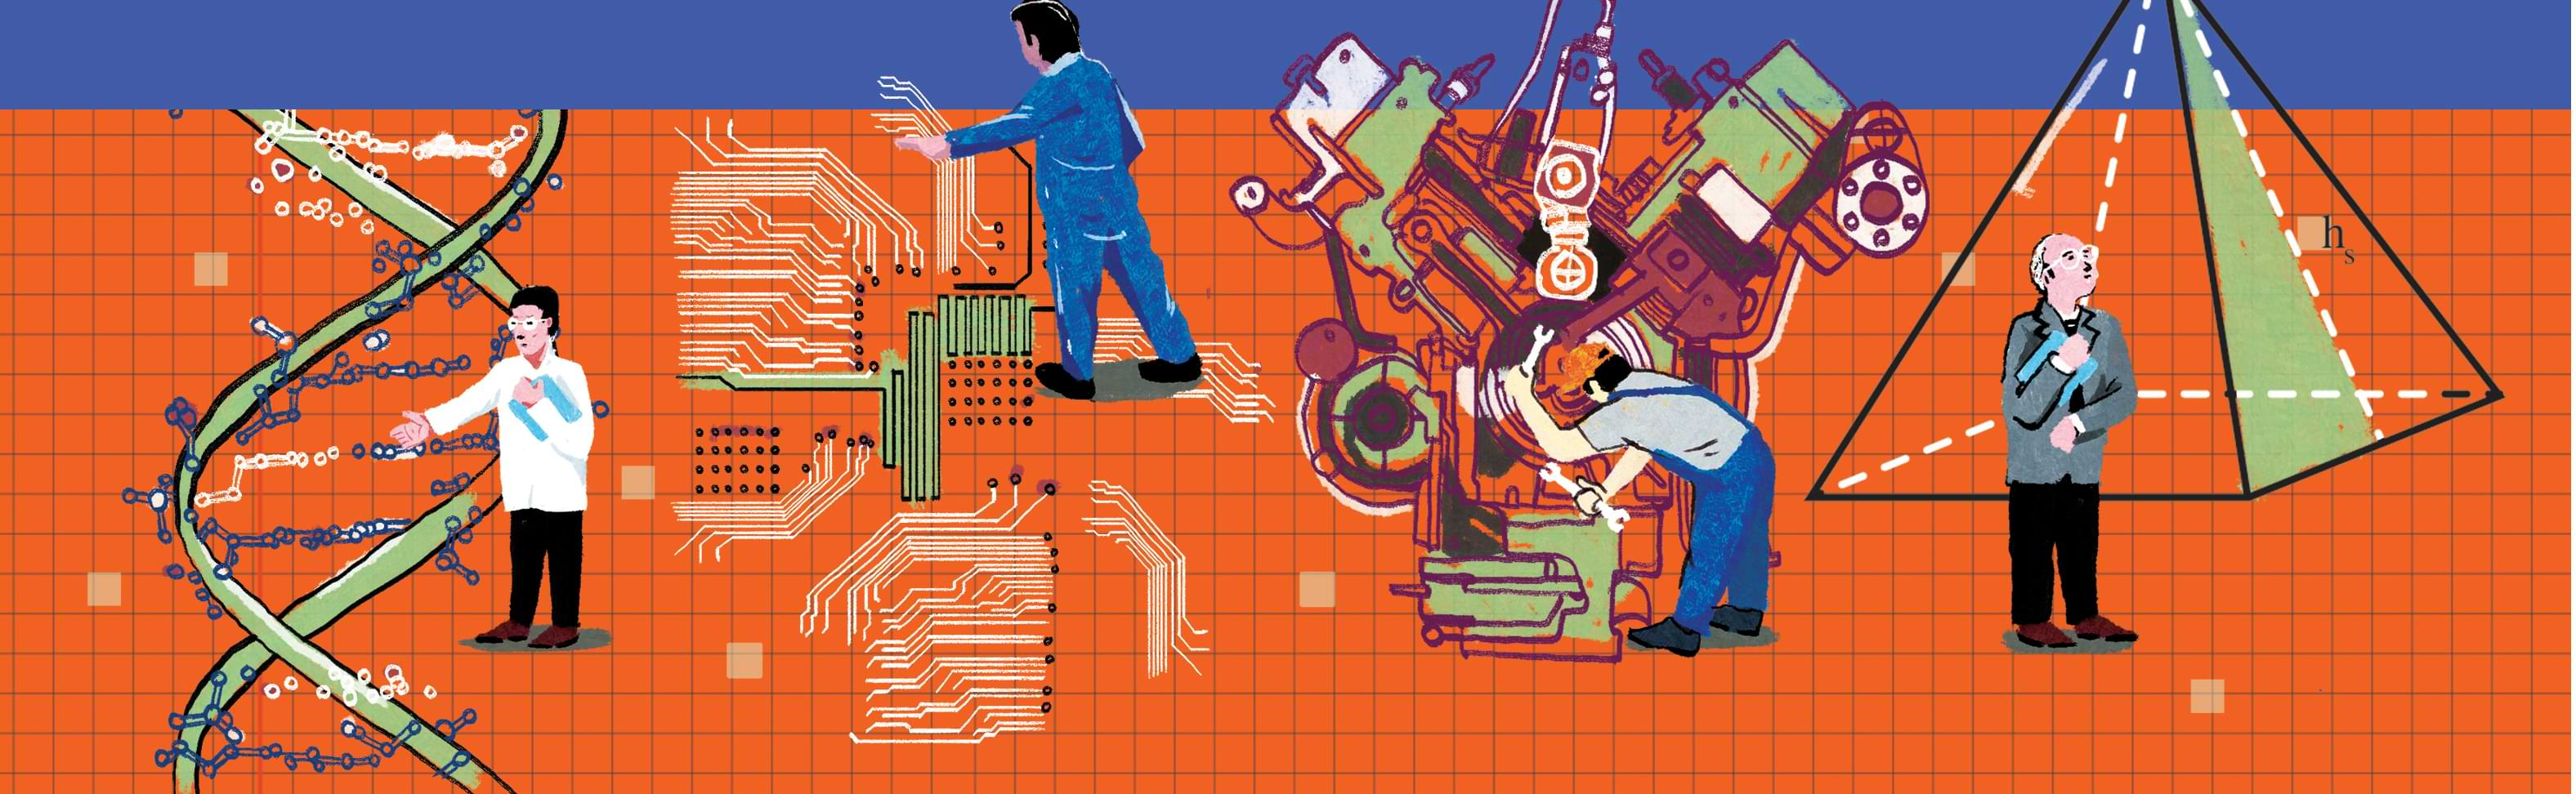
\includegraphics[width=19.3cm]{../bannertimhieu}}}
\AddToShipoutPicture*{\put(104,507){
\includegraphics[scale=1]{../tieude1.pdf}}}
\centering
\endgroup
\vspace*{198pt}

\begin{multicols}{2}
	Vườn thú Leipzig nằm ở bên kia rìa thành phố so với Viện Nhân chủng học Tiến hóa. Nhưng viện này có phòng thí nghiệm riêng trong khuôn viên, cũng như các phòng thử nghiệm được thiết kế đặc biệt bên trong ngôi nhà nghiên cứu về vượn, được gọi là Pongoland. Vì không ai trong số họ hàng Neanderthal gần nhất của chúng ta sống sót (ngoại trừ những mảnh DNA nhỏ trong chúng ta), các nhà nghiên cứu phải dựa vào họ hàng gần nhất của chúng ta là tinh tinh và bonobos, hay họ hàng xa hơn là khỉ đột và đười ươi -- để thực hiện các thí nghiệm sống. Một buổi sáng, tôi đến sở thú hy vọng sẽ xem một thí nghiệm đang được tiến hành.
	\begin{figure}[H]
		\vspace*{-5pt}
		\centering
		\captionsetup{labelformat= empty, justification=centering}
		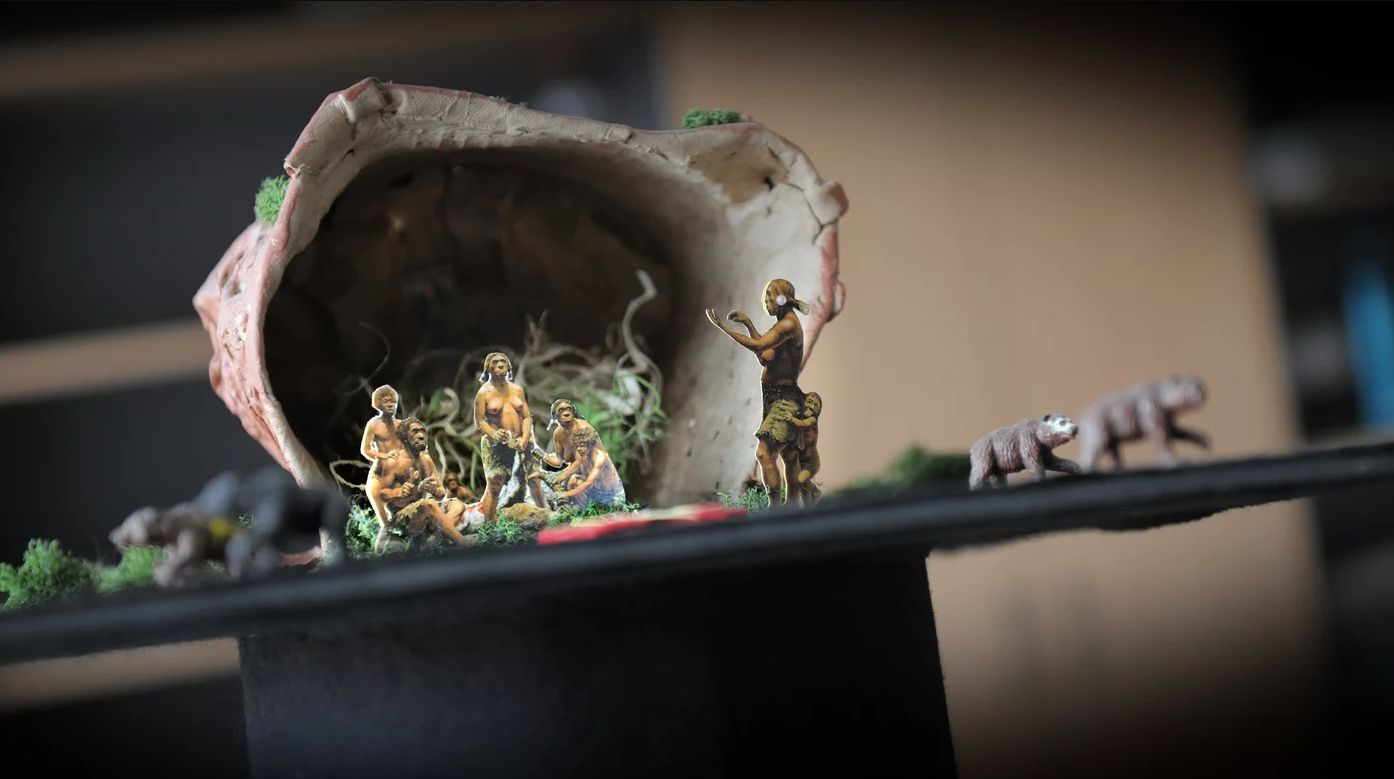
\includegraphics[width= 1\linewidth]{4}
		\caption{\small\textit{\color{timhieukhoahoc}Nhiều dữ liệu khảo cổ học đã hé lộ phần nào đời sống thường ngày của người Neanderthal hàng chục nghìn năm trước. Ảnh: mpg.de}}
		\vspace*{-5pt}
	\end{figure}
	Để lên hình cho đẹp, một nhà nghiên cứu tên là Héctor Marín Manrique chuẩn bị thực hiện lại một loạt các thí nghiệm khoa học mà ông đã làm. Một con đười ươi cái tên là Dokana được dẫn vào một trong những phòng thử nghiệm. Giống như hầu hết các con đười ươi khác, nó có bộ lông màu đồng và vẻ ngoài khinh khỉnh. Trong thí nghiệm đầu tiên liên quan đến nước trái cây màu đỏ và các ống nhựa nhỏ, Dokana có thể phân biệt ống hút nào thì dùng được và ống hút nào thì không. Trong phần thứ hai, có nhiều nước màu đỏ hơn và nhiều nhựa hơn, nó hiểu ý tưởng về ống hút bằng cách ngắt một đoạn của đường ống và dùng ống đó để hút nước. Cuối cùng, trong một màn thể hiện tài khéo léo ở cấp độ IQ cao thể hiện trí thông minh của loài vượn lớn, Dokana đã lấy được một hạt đậu phộng mà Manrique đã đặt ở đáy của một ống trụ dài. (Hình trụ được gắn cố định vào tường nên không thể dốc ngược ra). Nó đi đến chỗ uống nước, ngậm một ít nước trong miệng, trở lại và nhổ vào hình trụ, lặp lại quá trình cho đến khi hạt đậu phộng nổi đến tầm với của mình. Về sau, tôi thấy thí nghiệm này được dàn dựng lại với một số trẻ em năm tuổi sử dụng các hộp nhựa nhỏ hơn, những hạt đậu phộng được thay bằng kẹo. Mặc dù một bình đầy nước đã cố tình được để gần đó nhưng chỉ có một đứa trẻ -- một bé gái -- nghĩ ra phương án làm nó nổi lên và cũng phải sau một hồi gợi ý đủ kiểu (có bé trai còn hỏi ``Nước thì giúp con kiểu gì?", ngay trước khi bỏ cuộc).
	\vskip 0.1cm
	Một cách để cố gắng trả lời câu hỏi ``Điều gì làm nên con người chúng ta?" là hỏi ``Điều gì khiến chúng ta khác với loài vượn?" hoặc, nói chính xác hơn, với loài vượn khác (vì con người cũng thuộc nhóm vượn). Như tất cả mọi người giờ đây đã biết -- và như các thí nghiệm với Dokana một lần nữa khẳng định -- loài vượn khác cực kỳ thông minh. Chúng có khả năng suy luận, giải các câu đố phức tạp và hiểu những gì người khác có thể biết và không biết. Khi các nhà nghiên cứu từ Leipzig thực hiện một loạt các thử nghiệm trên tinh tinh, đười ươi và những đứa trẻ hai tuổi rưỡi, họ phát hiện ra rằng tinh tinh, đười ươi và những đứa trẻ khá tương đồng với nhau trong một loạt các hoạt động liên quan đến việc tìm hiểu về thế giới vật chất. Ví dụ: nếu một người thử nghiệm đặt phần thưởng vào một trong ba chiếc cốc, rồi tráo vị trí ba cốc này, thì loài vượn tìm ra phần thưởng cũng giỏi như lũ trẻ -- thậm chí, trong trường hợp của tinh tinh, còn giỏi hơn. Những con vượn dường như nắm bắt được khái niệm về số lượng tốt như lũ trẻ -- chúng luôn chọn chiếc đĩa chứa nhiều món hơn, thậm chí việc lựa chọn này cần dựa trên kỹ năng mà ta có thể tạm gọi là toán học -- và dường như loài vượn cũng nắm bắt tốt không kém bọn trẻ về quan hệ nhân quả. (Ví dụ, loài vượn hiểu rằng khi lắc một chiếc cốc mà chúng kêu lạo xạo thì khả năng cốc đó có thức ăn là cao hơn những chiếc cốc không phát ra tiếng động nào.) Và chúng cũng khôn khéo không thua gì trẻ em trong việc tận dụng các công cụ đơn~giản.
	\vskip 0.1cm
	Tuy nhiên, những đứa trẻ vượt trội hơn những con vượn ở điểm đọc các tín hiệu xã hội. Khi bọn trẻ được gợi ý về nơi tìm phần thưởng -- ai đó chỉ vào hoặc nhìn vào đúng hộp đựng -- lũ trẻ sẽ nhanh chóng bắt lấy cơ hội. Những con vượn thì hoặc là không hiểu chúng đang được giúp đỡ một tay, hoặc là không thể làm theo gợi ý. Tương tự, khi bọn trẻ được chỉ cách lấy phần thưởng, chẳng hạn như bằng cách xé toang hộp, chúng hiểu ý ngay và làm theo. Lũ vượn, một lần nữa, hết sức lúng túng. Phải thừa nhận rằng bọn trẻ có lợi thế lớn trong các hành động liên quan đến tương tác xã hội, vì chính những người thiết kế thí nghiệm cũng cùng giống loài với các em. Nhưng, nói chung, vượn dường như không có nhiều động lực để đạt được kỹ năng hợp tác cùng giải quyết vấn đề, vốn là trọng tâm của xã hội loài người.
	\vskip 0.1cm
	Michael Tomasello, người đứng đầu bộ phận tâm lý học so sánh và phát triển của viện, nói với tôi: ``Tinh tinh làm nhiều điều cực kỳ thông minh. Nhưng sự khác biệt chính [giữa con người và chúng] mà chúng tôi thấy là kỹ năng ‘ba cây chụm lại nên hòn núi cao’. Giờ đây nếu bạn quan sát ở sở thú, bạn sẽ không bao giờ thấy hai con tinh tinh cùng nhau khiêng vật nặng. Chúng không có kiểu hoạt động hợp tác như vậy".
	\begin{figure}[H]
		\vspace*{-5pt}
		\centering
		\captionsetup{labelformat= empty, justification=centering}
		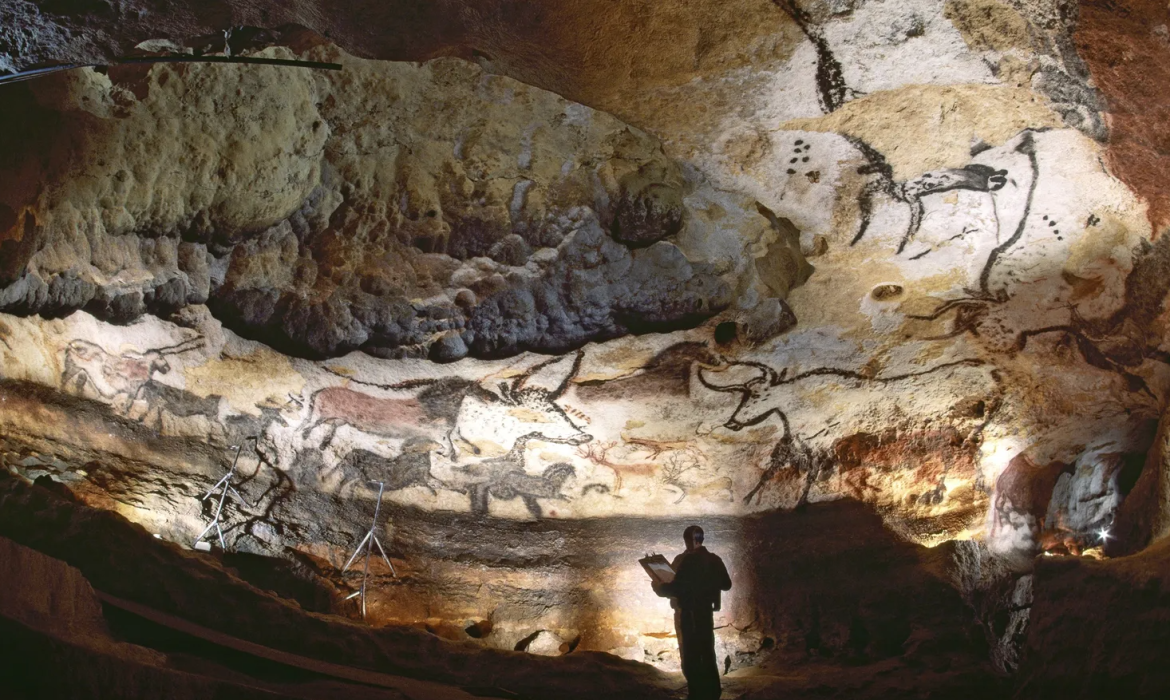
\includegraphics[width= 1\linewidth]{5}
		\caption{\small\textit{\color{timhieukhoahoc}Hang động Grotte des Combarelles trên vách tràn ngập các bức vẽ của người tối cổ. Điều gì thôi thúc con người len lỏi trong bóng tối mịt mù và chật hẹp để tạo nên những tác phẩm chưa chắc đã có người đồng cảm? Ảnh: National Geographic.}}
		\vspace*{-10pt}
	\end{figure}
	Trở về từ sở thú, tôi hỏi Pääbo về một thí nghiệm giả định. Nếu ông có cơ hội khiến người Neanderthal phải trải qua các loại bài kiểm tra mà tôi đã thấy ở Pongoland, ông sẽ làm gì? Ông ấy có nghĩ rằng mình có thể nói chuyện với họ không? Ông ngả người ra sau ghế và khoanh tay trước ngực.
	\vskip 0.1cm
	``Ai cũng không kìm được sự tò mò," ông nói. ``Vì vậy, tôi cố gắng kiềm chế điều đó bằng cách từ chối các câu hỏi như: `Họ có biết nói không?' Bởi vì, thực sự thì tôi không biết trả lời thế nào, và theo một cách nào đó, tôi cũng chỉ biết suy đoán như bạn mà thôi".
	\vskip 0.1cm
	Cho đến nay, rất nhiều địa điểm của người Neanderthal đã được khai quật, từ miền Tây Tây Ban Nha đến miền Trung nước Nga và từ Israel đến xứ Wales. Chúng cung cấp nhiều manh mối về người Neanderthal trông ra sao, ít nhất là với những người thích suy đoán. Người Neanderthal cực kỳ mạnh mẽ -- điều này được chứng thực bởi độ dày của xương họ -- và có thể đánh chúng ta nhừ tử cũng nên. Họ rất thành thạo trong việc chế tạo công cụ bằng đá, mặc dù có vẻ họ dành ra hàng chục nghìn năm chỉ để làm đi làm lại một vài công cụ, với những thay đổi không đáng kể. Ít nhất là trong một số trường hợp, họ chôn cất người đã khuất. Nhưng cũng trong một số trường hợp khác, họ có vẻ còn giết và ăn thịt lẫn nhau. Những vết nứt vỡ trên răng cửa của họ cho thấy họ đã rất mất công để dùng răng ngoạm da động vật, và điều này cũng gợi ý rằng họ đã xử lý da đó thành một loại da thuộc. Bộ xương của người Neanderthal thường để lại nhiều dấu vết của bệnh tật hoặc biến dạng. Ví dụ như người Neanderthal ban đầu của Mettmann, dường như đã phải trải qua và hồi phục từ hai vết thương nghiêm trọng, một ở đầu và một ở cánh tay trái. Người Neanderthal có bộ xương gần như hoàn chỉnh được tìm thấy ở La Chapelle đã phải chịu đựng ngoài việc bị viêm khớp còn bị gãy xương sườn và xương bánh chè ở đầu gối. Cả hai cá nhân này đều sống qua tuổi năm mươi, điều này cho thấy rằng người Neanderthal có khả năng hành động tập thể, hay nói cách khác mĩ miều hơn là có sự thấu cảm. Họ phải -- ít nhất là cũng có khi -- chăm sóc vết thương của đồng loại.
	\vskip 0.1cm
	Từ các nghiên cứu khảo cổ học, người ta suy ra rằng người Neanderthal tiến hóa ở Tây Á, chỉ dừng chân ở thủy vực hoặc gặp phải những trở ngại đáng kể nào đó khác. (Trong thời kỳ băng hà, mực nước biển thấp hơn rất nhiều so với hiện tại, vì vậy không có eo biển Anh để vượt qua). Đây là một trong những điểm cơ bản nhất mà con người hiện đại khác với người Neanderthal và, theo quan điểm của Pääbo, cũng là một trong những điều lý thú nhất. Vào khoảng bốn mươi lăm nghìn năm trước, con người hiện đại đã đặt chân đến Úc, một cuộc hành trình, kể cả ở giữa kỷ băng hà, cũng có nghĩa là băng qua vùng nước mở. Những con người cổ đại như Homo erectus ``chỉ đi loanh quanh như rất nhiều loài động vật có vú khác ở thời Cựu Thế giới," Pääbo nói với tôi. ``Họ không bao giờ đến Madagascar, không bao giờ đến Úc. Người Neanderthal cũng vậy. Chỉ có những con người hoàn toàn hiện đại mới bắt đầu hành trình mạo hiểm trên đại dương, nơi người ta không nhìn thấy đất liền. Tất nhiên, một phần là nhờ công nghệ; bạn phải có tàu để làm điều đó. Nhưng tôi thích nghĩ và nói rằng, còn cần một chút ``điên rồ" nữa. Bạn biết không, biết bao nhiêu người hẳn đã ra khơi và biến mất trên Thái Bình Dương trước khi đặt chân được đến đảo Phục Sinh? Ý tôi là, điều đó thật nực cười. Và tại sao người ta lại dám làm thế? Có phải vì vinh quang? Vì sự bất tử? Vì tò mò? Giờ đây chúng ta còn đòi lên sao Hỏa nữa. Đúng là không biết điểm dừng". Nếu đặc tính của con người hiện đại là sự thao thức, ``không bao giờ bằng lòng với hiện tại" của nhân vật Faust trong vở kịch của Goethe, hẳn phải có một loại gene Faust nào đó trong chúng ta, theo quan điểm của Pääbo. Rất nhiều lần, ông nói với tôi rằng có thể xác định được nguyên nhân của sự ``điên rồ" này bằng cách so sánh DNA của Neanderthal và con người.
	\vskip 0.1cm
	``Nếu một ngày nào đó chúng ta biết được rằng một số đột biến kỳ lạ đã làm nên sự điên rồ và thích khám phá mọi thứ của con người, thì sẽ thật ảo diệu khi nghĩ rằng chỉ một chút xáo trộn này trên nhiễm sắc thể kia mà đã tạo nên ngày hôm nay, đã thay đổi toàn bộ hệ sinh thái trên hành tinh này và khiến chúng ta thống trị tất cả".
	\vskip 0.2cm
	\PIbox{Nếu đặc tính của con người hiện đại là sự thao thức, ``không bao giờ bằng lòng với hiện tại" của nhân vật Faust trong vở kịch của Goethe, hẳn phải có một loại gene Faust nào đó trong chúng ta, theo quan điểm của Pääbo.}
	\vskip 0.2cm
	Theo những ước tính gần đây nhất, người Neanderthal và người hiện đại có chung một tổ tiên sống cách đây khoảng bốn trăm nghìn năm. (Không rõ tổ tiên đó là ai, mặc dù có một khả năng là loài hominid nào đó mới được biết đến một cách mơ hồ, sau khi người ta tìm thấy một xương hàm ở gần Heidelberg, với tên gọi Homo heidelbergensi). Còn tổ tiên chung của tinh tinh và người, sống cách đây năm đến bảy triệu năm trước. Điều này có nghĩa là người Neanderthal và con người có ít hơn $1/10$ thời gian đó để tích lũy sự khác biệt về gene.
	\begin{figure}[H]
		\vspace*{-5pt}
		\centering
		\captionsetup{labelformat= empty, justification=centering}
		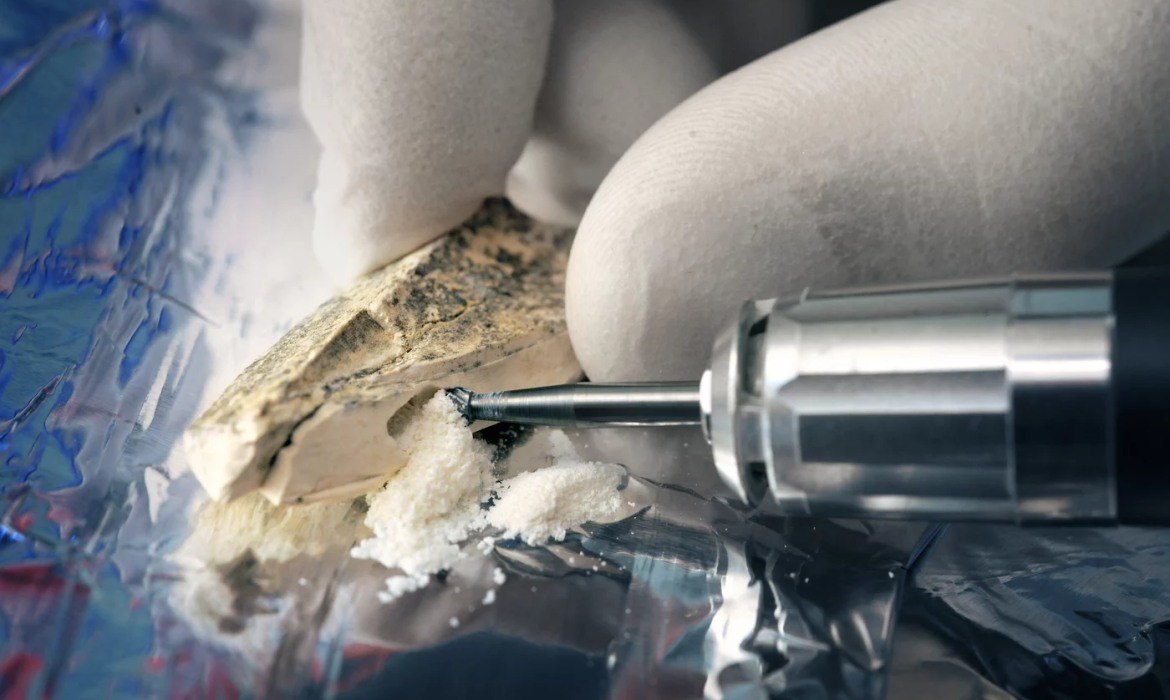
\includegraphics[width= 1\linewidth]{6}
		\caption{\small\textit{\color{timhieukhoahoc}Người ta cần khoảng $400$ mg bột xương để thực hiện một phân tích gene. Nhưng nhiều khi kết quả không chỉ gồm gene của người Neanderthal mà còn tạp nhiễm cả của vi sinh vật. Ảnh: mpg.de}}
		\vspace*{-10pt}
	\end{figure}
	Về nguyên tắc, việc lập bản đồ những khác biệt này khá đơn giản về lý thuyết. Còn trong thực tế, nó phức tạp hơn một chút. Để bắt đầu, thực sự không có cái gọi là bộ gene chung của con người; ai cũng có bộ gene của riêng mình và chúng khác nhau đáng kể -- giữa bạn và người ngồi cạnh bạn trên tàu điện ngầm, sự khác biệt rất có thể là đâu đó khoảng ba triệu cặp cơ bản. Một số biến thể này tương ứng với những khác biệt sinh lý có thể nhìn thấy -- chẳng hạn như màu mắt, hoặc khả năng mắc bệnh liên quan đến tim mạch -- và một số khác không có ý nghĩa đáng kể. Theo ước tính đầu tiên, một người và một người Neanderthal bất kỳ cũng sẽ khác nhau ba triệu cặp cơ sở. Cái khó là xác định chắc chắn cái nào trong số hàng triệu biến thể này đã tách chúng ta khỏi họ. Pääbo ước tính rằng khi Dự án bộ gene người Neanderthal hoàn thành, danh sách các cặp cơ bản độc nhất của con người với người Neanderthal sẽ đâu đó khoảng một trăm nghìn cặp. Đâu đó trong danh sách này sẽ ẩn giấu sự thay đổi -- hay những thay đổi -- đã khởi tạo nên chúng ta. Để xác định những đột biến gene này, ông cần phải nhờ đến những con chuột chuyển~gene.
	\vskip 0.1cm
	Từ quan điểm thực nghiệm, cách tốt nhất để kiểm tra xem thay đổi gene nào mới đáng kể là tạo ra một con người với trình tự gene của người Neanderthal. Điều này sẽ liên quan đến việc chỉnh sửa tế bào gốc của người, cấy phôi đã biến đổi gene đó vào một phụ nữ mang thai hộ và rồi quan sát đứa trẻ của thí nghiệm đó lớn lên. Vì những lý do quá rõ ràng, không ai cho phép một thí nghiệm trên người như vậy, đó còn chưa kể là nó còn bất khả. Vì những lý do tương tự, thí nghiệm kiểu này cũng không được phép áp dụng trên tinh tinh. Nhưng trên chuột thì được. Hàng chục giống chuột đã được chỉnh sửa gene để mang các trình tự gene của người, và người ta vẫn tạo ra các giống mới liên tục, đặt hàng khá dễ dàng.
	\vskip 0.1cm
	Vài năm trước, Pääbo và một đồng nghiệp, Wolfgang Enard, bắt đầu quan tâm đến một gene được gọi là FOXP$2$, gene này ở người có liên quan đến ngôn ngữ. (Những người có một bản sao gene bị lỗi -- một trường hợp cực kỳ hiếm xảy ra -- có khả năng nói, nhưng những gì họ nói, đối với người lạ, hầu như không thể hiểu được.) Pääbo và Enard đã nuôi một số con chuột với một phiên bản gene này, và sau đó nghiên cứu chúng từ mọi góc độ có thể. Những con chuột bị biến đổi, có giọng kêu trầm hơn so với các đồng loại chưa được ``nhân hóa" của chúng. Những con chuột này cũng thể hiện sự khác biệt đáng kể về phát triển thần kinh. Gene FOXP$2$ của người Neanderthal, hóa ra, gần như giống hệt loài người, khác có mỗi một cặp cơ bản. Khi ông phát hiện ra sự khác biệt này, ông đặt hàng ngay một lô chuột chuyển gene mới mà lúc tôi tới thăm phòng thí nghiệm của ông, vừa mới sinh ra và đang được nuôi trong điều kiện tiệt trùng dưới tầng hầm.
	\vskip 0.1cm
	Các gene liên quan đến kỹ năng nói của chúng ta là địa chỉ hiển nhiên để tìm kiếm những thay đổi khiến chúng ta là con người. Nhưng lý do của việc phải giải trình tự toàn bộ hệ gene của người Neanderthal là bởi địa chỉ hiển nhiên nhất chưa chắc đã là địa chỉ đúng nhất.
	\vskip 0.1cm
	Pääbo nói với tôi: ``Ưu điểm tuyệt vời của nghiên cứu gene theo phương thức này là nó không có thiên kiến. Nếu bạn chỉ chạy theo những gene ứng cử viên, bạn sẽ dễ phát biểu cảm tính rằng gene này hay gene kia mới là quan trọng nhất. Nhiều người sẽ bảo là gene ngôn ngữ. Nhưng có khi chúng ta sẽ ngạc nhiên vì gene khác mới là cốt yếu". Gần đây, Pääbo trở nên hứng thú với một gene có tên là RUNX$2$, liên quan đến quá trình hình thành xương. Khi các thành viên trong nhóm của ông phân tích toán học bộ gene người và người Neanderthal, RUNX$2$ bỗng nổi lên như một vị trí đánh dấu sự rẽ nhánh của những dòng dõi người.
	\vskip 0.1cm
	Những người có bản sao bị lỗi của gene RUNX$2$ thường phát triển một tình trạng, được gọi là chứng loạn sản xương sọ, có các triệu chứng bao gồm các đặc điểm bề ngoài giống người Neanderthal như khung xương sườn loe ra. Hai gene có liên quan đến chứng tự kỷ, CADPS$2$ và AUTS$2$, dường như có sự khác biệt đáng kể giữa người Neanderthal và người. Điều này rất thú vị vì một trong những triệu chứng của chứng tự kỷ là không có khả năng đọc các tín hiệu xã hội.
	\vskip 0.1cm
	Vào một buổi chiều nọ, khi tôi đi lang thang trong văn phòng của ông, Pääbo cho tôi xem một bức ảnh chụp nắp sọ mới được một nhà sưu tập nghiệp dư phát hiện cách Leipzig khoảng nửa giờ. Từ bức ảnh đã được gửi qua email, Pääbo nhận định rằng chiếc xương sọ có thể là đồ cổ -- từ thời sơ khai của người Neanderthal, hoặc thậm chí là người Homo heidelbergensis. Ông cũng quyết định phải có nó bằng được. Chiếc nắp sọ đã được tìm thấy tại một mỏ đá trong một hố nước -- ông giả thiết rằng có lẽ những điều kiện này đã bảo quản nó, và nếu ông nhanh chóng kịp đưa nó về, ông có thể trích xuất một số DNA. Nhưng hộp sọ đã được hứa đưa tới một giáo sư nhân chủng học ở Mainz trước. Làm thế nào mà Pääbo thuyết phục người giáo sư để lại cho ông đủ xương để kiểm nghiệm bây~giờ?
	\vskip 0.1cm
	Pääbo gọi cho tất cả những người mà ông nghĩ biết đâu có thể quen với giáo sư kia. Ông còn yêu cầu thư ký của mình liên hệ với thư ký của giáo sư kia để xin số điện thoại cá nhân và nói đùa -- có khi nửa đùa nửa thật cũng nên -- rằng nếu cần thiết thì Pääbo sẵn sàng ``bán thân" cho giáo sư luôn. Cuộc gọi điện thoại qua lại điên cuồng trên khắp nước Đức kéo dài hơn một tiếng rưỡi đến khi cuối cùng Pääbo quay ra nói chuyện với một nhà nghiên cứu cùng lab với mình. Nhà nghiên cứu này hóa ra đã tận mắt nhìn thấy chiếc nắp sọ thực sự và kết luận miếng xương này khả năng cao là không phải đồ cổ gì cho lắm. Pääbo ngay lập tức không còn hứng thú gì với nó nữa.
	\vskip 0.1cm
	Với những bộ xương cổ, không ai thực sự biết trước có thể thu được thông tin gì từ nó. Cách đây vài năm, Pääbo lấy được một phần răng từ một trong những bộ xương được gọi là ``người Hobbit" được tìm thấy trên đảo Flores, Indonesia. (``Người Hobbit", được phát hiện vào năm $2004$, thường được cho là loài người cổ đại thấp bé -- Homo floresiensis -- mặc dù một số nhà khoa học đã lập luận rằng đó chỉ là người hiện đại bị chứng teo não.) Chiếc răng, khoảng $17$ nghìn năm tuổi, không chứa một chút DNA nào.
	\vskip 0.1cm
	Sau đó, khoảng một năm rưỡi trước, Pääbo đã lấy được một mảnh xương ngón tay được khai quật trong một hang động ở miền Nam Siberia cùng với một chiếc răng hàm kỳ dị, trông có vẻ giống người. Xương ngón tay -- có kích thước bằng cục tẩy bút chì -- được cho là đã hơn bốn vạn năm tuổi. Pääbo cho rằng nó đến từ người hiện đại hoặc từ người Neanderthal. Nếu điều này là đúng, thì địa điểm đó sẽ là nơi xa nhất về phía Đông mà người ta tìm thấy hài cốt người Neanderthal.
	\vskip 0.1cm
	Trái ngược với chiếc răng của người Hobbit, đoạn ngón tay mang lại một lượng DNA lớn đáng kinh ngạc. Khi việc phân tích các mẩu thông tin đầu tiên được hoàn thành, Pääbo tình cờ lúc đó đang ở Hoa Kỳ. Ông gọi điện đến văn phòng và một trong những đồng nghiệp của ông trả lời: ``Ông đang ngồi chắc chắn trên ghế chứ?" DNA cho thấy dữ liệu không thể thuộc về người Neanderthal hoặc của người hiện đại. Thay vào đó, chủ nhân của nó phải thuộc về một loài hominid hoàn toàn khác và chưa từng được phát hiện ra trước đó. Trong một bài báo được xuất bản vào tháng $12/2010$, trên tạp chí Nature, Pääbo và nhóm của ông đã đặt tên cho nhóm này là người Denisovan, theo tên của hang Denisova, nơi xương đã được tìm thấy. Tờ \textit{Sydney Morning Herald} chạy tít: ``Một ngón tay đóng dấu lịch sử cổ đại của con người". Thật đáng kinh ngạc -- hay có lẽ, giờ đây, người ta cũng đã đoán được -- con người hiện đại hẳn đã phối ngẫu với cả người Denisovan bởi vì những người New Guinean ngày nay mang tới $6\%$ DNA của người Denisovan. (Tại sao điều này đúng với người New Guinea nhưng không phải với người Siberia bản địa hoặc người châu Á thì chưa rõ, nhưng có lẽ liên quan đến các mẫu hình di cư của con người).
	\vskip 0.1cm
	Từ lâu, người ta đã hiểu rằng con người hiện đại và người Neanderthal là những người sống cùng thời với nhau. Việc phát hiện ra người Hobbit và bây giờ là người Denisovan cho thấy con người đã chia sẻ hành tinh với ít nhất hai sinh vật khác giống như chúng ta. Và có vẻ như càng phân tích DNA từ các bộ hài cốt cổ đại thì sẽ càng thấy những loài khác có họ hàng với người; như Chris Stringer, một nhà cổ sinh vật học nổi tiếng người Anh, đã nói với tôi, ``Tôi chắc chắn rằng chúng ta sẽ có thêm nhiều điều bất ngờ nữa đang đến."
	\vskip 0.1cm
	``Nếu những dạng người khác này tồn tại được hơn hai nghìn thế hệ nữa, tức là không quá lâu, thì điều đó sẽ ảnh hưởng như thế nào đến quan điểm của chúng ta về thế giới sinh vật?" Pääbo nói, khi sự phấn khích với câu chuyện về xương nắp sọ đã chùng xuống và chúng tôi ngồi uống cà phê với nhau. ``Chúng ta từng đặt ra một ranh giới rõ ràng giữa con người và động vật. Nhưng có thể ranh giới đó không rõ ràng đến thế. Đó là một điều thú vị để triết lý." Cũng thật thú vị khi nghĩ về lý do tại sao chúng ta là những người sống sót.
	\vskip 0.1cm
	Trong nhiều thập kỷ, nhiều giả thuyết đã được đưa ra để giải thích nguyên nhân gây ra sự diệt vong của người Neanderthal, từ biến đổi khí hậu cho đến vận rủi đơn thuần. Tuy nhiên, trong những năm gần đây, ngày càng rõ ràng rằng, như Pääbo đã nói với tôi, ``vận rủi của họ là chính chúng ta". Hết lần này đến lần khác, bằng chứng khảo cổ học ở châu Âu chỉ ra rằng, mỗi khi con người hiện đại xuất hiện ở nơi nào người Neanderthal đang sinh sống, thì người Neanderthal ở vùng đó sẽ biến mất. Có thể người Neanderthal đã bị truy đuổi ráo riết, hoặc có lẽ họ đã bị thua trong cuộc cạnh tranh sinh tồn. ``Vận rủi" của người Neanderthal có lẽ giống với bất hạnh mà người Hobbit và người Denisovan gặp phải, và tương tự như thảm kịch mà các loài thú có túi khổng lồ từng thống trị khắp Australia, và một loạt các loài thú lớn từng sinh sống ở Bắc Mỹ, những con chim Moa từng sống ở New Zealand. Và chính sự xui xẻo đó đã đưa rất nhiều loài -- trong đó có tất cả các loài vượn lớn -- đến bờ vực của sự lãng quên ngày nay.
	\begin{figure}[H]
		\vspace*{-5pt}
		\centering
		\captionsetup{labelformat= empty, justification=centering}
		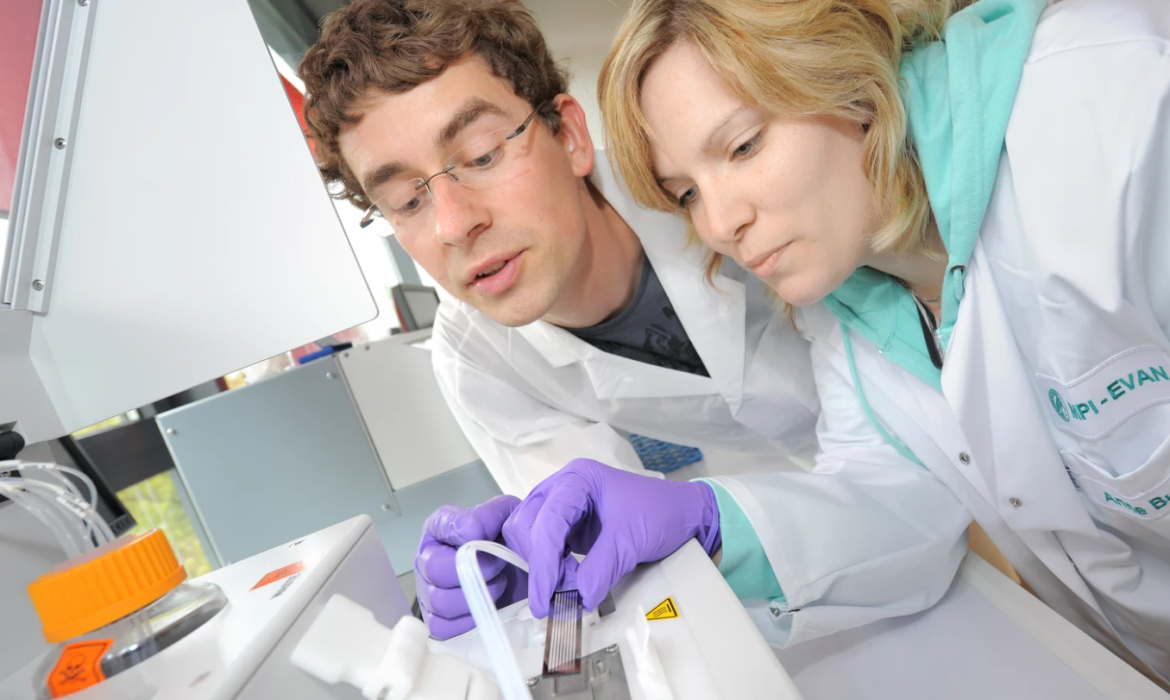
\includegraphics[width= 1\linewidth]{7}
		\caption{\small\textit{\color{timhieukhoahoc}Hai thành viên trong phòng thí nghiệm của Svante Pääbo đang chạy máy phân tích genome. Nó có thể phân tích cùng lúc nhiều mẫu. Ảnh: mpg.de}}
		\vspace*{-10pt}
	\end{figure}
	``Đối với tôi, sự tuyệt chủng của người Neanderthal không phải là điều bí ẩn", Jean--Jacques Hublin, giám đốc bộ phận tiến hóa của con người thuộc Viện Nhân chủng học Tiến hóa, nói với tôi. ``Đối với tôi, bí ẩn là điều gì khiến loài người hiện đại trở thành một nhóm thành công đến mức họ đã thay thế không chỉ người Neanderthal mà còn tất cả mọi thứ. Chúng tôi không có mấy bằng chứng cho thấy người Neanderthal hoặc những con người cổ xưa khác đã đẩy một loài thú có vú hoặc bất cứ thứ gì khác đến bờ vực tuyệt chủng. Còn với con người hiện đại thì có hàng trăm ví dụ, và chúng ta đã làm điều đó hết sức thành thục".
	\vskip 0.1cm
	Một trong số những tập hợp xương người Neanderthal lớn nhất từng được tìm thấy -- hài cốt của bảy cá thể -- được phát hiện cách đây khoảng một thế kỷ tại một địa điểm được gọi là La Ferrassie, Tây Nam nước Pháp. La Ferrassie nằm ở Dordogne, không xa La Chapelle và cách hàng chục địa điểm khảo cổ quan trọng khác trong vòng nửa giờ lái xe, bao gồm cả các hang động được sơn ở Lascaux. Trong mùa hè, một nhóm bao gồm một trong những đồng nghiệp của Pääbo đang khai quật tại La Ferrassie, và tôi quyết định xuống đó để quan sát. Tôi đến trụ sở của nhóm khai quật -- một kho thuốc lá đã được chuyển đổi mục đích -- đúng lúc đang họ dùng bữa tối với món bò hầm rượu vang, được phục vụ trên những chiếc bàn tạm ở sân sau.
	\vskip 0.1cm
	Ngày hôm sau, tôi lái xe đến La Ferrassie cùng với một số nhà khảo cổ học của nhóm. Địa điểm này nằm trong một khu vực nông thôn yên bình, ngay bên đường. Nhiều nghìn năm trước, La Ferrassie là một hang động đá vôi khổng lồ, nhưng một trong những vách hang bị đổ sập xuống, và có tới hai lối vào. Một phiến đá khổng lồ nhô lên khỏi mặt đất khoảng $6$ m, hình vòng cung. Người ta rào dây quanh khu vực đào bới trông nó có dáng dấp như hiện trường của một vụ án mạng.
	\vskip 0.1cm
	Ngày hôm đó nắng nóng và bụi bặm. Nửa tá sinh viên chui rúc trong rãnh dài, dùng bay bới đất. Dọc theo thành rãnh, tôi có thể nhìn thấy những mảnh xương nhô ra từ đất đỏ. Người ta nói với tôi, những mẩu xương ở gần đáy là do người Neanderthal ném xuống. Phần xương gần đỉnh là những gì người hiện đại để lại, những người đã chiếm đóng La Ferrassie sau khi người Neanderthal biến mất. Các bộ xương của người Neanderthal ở đây đã bị mang đi từ lâu, nhưng người ta vẫn hy vọng rằng biết đâu vẫn tìm được một số mảnh vụn còn sót lại, chẳng hạn như một chiếc răng. Mỗi mảnh xương được khai quật cùng với mảnh đá lửa và bất cứ thứ gì khác có tiềm năng quan tâm sẽ được đặt sang một bên, đưa về trụ sở chính để phân loại và gắn~thẻ.
	\vskip 0.1cm
	Sau khi thấy các sinh viên trở nên thấm mệt, tôi lui vào bóng râm. Tôi cố tưởng tượng cuộc sống của người Neanderthal ở La Ferrassie sẽ như thế nào. Mặc dù khu vực này giờ đây tràn ngập cây cỏ, nhưng trước đấy nó hẳn là lãnh nguyên. Sẽ có nai sừng tấm đi lang thang trong thung lũng, tuần lộc, gia súc hoang dã và voi ma mút. Ngoài những chi tiết rời rạc này, tôi không thể nghĩ được điều gì khác. Tôi đem điều đó tới hỏi những nhà khảo cổ đi cùng.
	\vskip 0.1cm
	``Rất lạnh," Shannon McPherron, thuộc Viện Max Planck, phát biểu đầu tiên.
	\vskip 0.1cm
	``Và hôi hám", Dennis Sandgathe, thuộc Đại học Simon Fraser của Canada, cho biết.
	\vskip 0.1cm
	``Có lẽ là họ phải chịu đói," Harold Dibble, Đại học Pennsylvania, nói thêm.
	\vskip 0.1cm
	Sandgathe nói: ``Không ai sống nổi đến già cả".
	\vskip 0.1cm
	Sau đó, trở lại nhà kho, tôi nhặt lên xem những gì đã đào được trong vài ngày qua. Có hàng trăm mảnh xương động vật, mỗi mảnh đều được làm sạch và đánh số thứ tự rồi được đặt trong túi nhựa nhỏ của riêng nó, và hàng trăm mảnh đá lửa. Hầu hết các mảnh này có lẽ là sản phẩm phụ của quá trình chế tạo công cụ -- tạm gọi là dăm bào thời kỳ Đồ đá -- nhưng một số mảnh, tôi biết được, chính là công cụ. Từng được hướng dẫn cách nhìn những thứ đồ này, tôi có thể thấy các cạnh vát mà người Neanderthal đã chế tác. Một công cụ đặc biệt nổi bật: một viên đá lửa cỡ lòng bàn tay có hình giọt nước. Theo thuật ngữ khảo cổ học, nó là một cái rìu cầm tay, mặc dù nó có lẽ không được dùng như một cái rìu theo nghĩa hiện nay. Nó đã được tìm thấy gần đáy của rãnh, vì vậy nó được ước tính là khoảng $70$ nghìn năm tuổi. Tôi lấy nó ra khỏi túi nhựa và lật đi lật lại. Nó gần như đối xứng hoàn hảo và -- ít nhất là đối với mắt thường -- khá đẹp. Tôi nói rằng tôi nghĩ người Neanderthal đã tạo ra nó hẳn là người có khiếu thiết kế tốt. McPherron phản đối.
	\vskip 0.1cm
	``Chúng ta biết câu chuyện kết thúc thế nào", anh ấy nói với tôi. ``Chúng ta biết về văn hóa hiện đại ngày nay và chúng ta tò mò tại sao chúng ta trở nên như vậy. Và ta có xu hướng phóng đại những gì ở quá khứ bằng cách nhìn nó với con mắt người hiện đại. Vì vậy, khi bạn nhìn thấy một chiếc rìu cầm tay đẹp và bạn nói, ‘Ôi nhìn trình độ chế tác của nó này, thực sự là một tác phẩm nghệ thuật". Đó là quan điểm của người ngày nay. Bạn không thể đưa ra kết luận về thứ mà bạn đang cố gắng chứng minh".
	\vskip 0.1cm
	Trong số hàng trăm nghìn đồ tạo tác của người Neanderthal đã được khai quật, hầu như không có đồ vật nào đại diện cho những ý đồ rõ ràng về mục đích nghệ thuật hoặc trang trí, và những đồ vật được giải thích theo cách này -- ví dụ, mặt dây chuyền bằng ngà voi được phát hiện trong một hang động ở miền Trung nước Pháp -- chỉ khơi mào cho những cuộc tranh cãi mơ hồ và không đi đến đâu. (Nhiều nhà khảo cổ học tin rằng mặt dây chuyền được tạo ra bởi người Neanderthal, những người đã tiếp xúc với người hiện đại và cố gắng bắt chước họ, nhưng, dựa trên các kỹ thuật xác định niên đại gần đây nhất, một số người cho rằng mặt dây chuyền thực tế là do người hiện đại tạo ra.) Sự thiếu bằng chứng này đã khiến một số người cho rằng người Neanderthal không có khả năng nghệ thuật hoặc không quan tâm đến nó. Đơn giản là họ không sở hữu thứ, về mặt di truyền học, có thể được gọi là đột biến thẩm mỹ.
	\vskip 0.1cm
	Vào ngày cuối cùng của tôi ở Dordogne, Pháp, tôi quyết định đến thăm một địa điểm gần đó về con người được biết đến với những hình ảnh phi thường. Địa điểm, Grotte des Combarelles, là một hang động dài, rất hẹp, ngoằn ngoèo xuyên qua một vách núi đá vôi. Sâu trong đó dăm chục mét, các bức tường của hang động được bao phủ bởi các hình chạm khắc -- một con voi ma mút đang thu vòi lại, một con ngựa hoang đang vươn cao đầu, một con tuần lộc đang rướn người về phía trước, dường như để uống nước. Mới gần đây thôi, người ta đào sàn của Grotte des Combarelles thành rãnh, vừa đủ để một người có thể đi bộ trong đó và đường hầm được được chiếu sáng lờ mờ bởi đèn điện. Nhưng khi các bản khắc ban đầu được tạo ra, khoảng mười hai hoặc mười ba nghìn năm trước, cách duy nhất để vào được đây là phải bò và cách duy nhất để nhìn trong bóng tối đen như mực là phải mang theo đuốc. Khi tôi quờ quạng trong bóng tối, lướt qua những bản khắc về bò rừng wisent và bò rừng aurochs và tê giác lông mượt, tôi bỗng nhận ra rằng mình hoàn toàn không tưởng tượng được điều gì đã thôi thúc ai đó phải luồn lách qua một đường hầm tối tăm để bao phủ vách hang bằng những bức tranh mà chỉ ai cũng phải đồng cảm và mạo hiểm tương tự mới chiêm ngưỡng được. Và một xúc cảm dội vào tôi khi chứng kiến những gì là đặc trưng của con người đang hiển hiện -- sự sáng tạo, sự táo bạo, ``sự điên rồ". Và tôi nghĩ về cả những con vật được vẽ trên vách hang -- những con bò rừng, voi ma mút và tê giác. Những con quái thú khổng lồ này phải chạy trốn khỏi sự săn bắn truy đuổi của những người châu Âu thời kỳ Đồ đá cũ, và rồi, từng con một, cùng với những người Neanderthals, bị tận diệt.
	\vskip 0.1cm
	\textbf{{\color{timhieukhoahoc}Nguyên tác:}} \hspace*{5pt} {\small\url{https://www.newyorker.com/magazine/2011/08/15/sleeping-with-the-enemy}}
\end{multicols}
\vspace*{-10pt}
{\color{timhieukhoahoc}\rule{1\linewidth}{0.1pt}}

\vspace*{10pt}
\centerline{\textbf{\LARGE\color{timhieukhoahoc}LỜI GIẢI, ĐÁP ÁN}}
\vskip 0.1cm
\begin{multicols}{2}
	\textbf{\color{timhieukhoahoc}Đố vui} 
	\vskip 0.1cm
	Vì $10$ cô gái nhận có số lần nhận được nón nhiều hơn số lần chuyển nón đi nên các cô gái này đã cầm nón lên sân khấu và kết thúc tiết mục mà không cầm nón. Mười chiếc nón mà họ mang lên sân khấu phải được $10$ cô gái khác cầm khi tiết mục kết thúc. Mà có tiết mục có đúng $20$ cô gái nên không còn cô gái nào khác và chiếc nón nào khác. Nghĩa là có đúng $10$ cô gái đã cầm nón lên sân khấu. 
	\vskip 0.1cm
	\textbf{\color{timhieukhoahoc}Một cuộc thẩm vấn đặc biệt}
	\vskip 0.1cm
	Các em xét hai trường hợp sau đây: ông Kim và ông Lee làm ở cùng một công ty hoặc họ làm ở hai công ty khác nhau.
	\vskip 0.1cm
	Trường hợp đầu tiên, nếu ông Kim và ông Lee cùng làm ở một công ty, thì do họ nói thật với nhau, suy ra ông Kim làm ở công ty Sungsang. Nhưng vì ông Lee cũng nói thật, suy ra ông Han và ông Kim cùng làm ở công ty Sungsang.
	\vskip 0.1cm
	Trường hợp thứ hai, nếu họ làm khác công ty, thì ông Kim đã nói dối ông Lee, vì thế thực ra ông Kim làm ở công ty TungTeng. Nhưng do ông Lee cũng nói dối ông Kim, nên ông Kim và ông Han phải làm ở các công ty khác nhau. Vì ông Kim làm việc ở công ty TungTeng, nên ông Han làm việc ở công ty Sungsang.
	\vskip 0.1cm
	Như vậy, trong mọi trường hợp, ông Han luôn làm việc ở công ty Sungsang.
	\vskip 0.1cm
	\textbf{\color{timhieukhoahoc}Góc cờ}
	\vskip 0.1cm
	$\pmb{1}$\textbf{\color{timhieukhoahoc}.Hc$\pmb{6+}$ Va}$\pmb{7}$ [$1$...Xb$6$ $2$.Ha$8+$ Vb$5$ $3$.Vb$3!$ Xa$6$ $4$.Hd$5+$ Vb$6$ $5$.Va$4$]
	\vskip 0.1cm
	$\pmb{2}$\textbf{\color{timhieukhoahoc}.Vd}$3$! [Vì xe đen chỉ có $1$ điểm tựa an toàn nhất là b$4$ nên đến lúc này họ bắt buộc phải di chuyển xe]
	\vskip 0.1cm
	$\pmb{2}$\textbf{\color{timhieukhoahoc}...Xb$\pmb{6}$ $\pmb{3}$.Hc$\pmb{7+}$ Va$\pmb{6}$ $\pmb{4}$.Hc$\pmb{8+}$ Va}$\pmb{7}$ [$\pmb{4}$...Vb$\pmb{5}$ $\pmb{5}$.Hc$\pmb{4\#}$]
	\vskip 0.1cm
	$\pmb{5}$\textbf{\color{timhieukhoahoc}.Vc$\pmb{4}$ Xb$\pmb{7}$ $\pmb{6}$.Hd$\pmb{8}$ Va$\pmb{6}$ $\pmb{7}$.Vc$\pmb{5}$ Xb$\pmb{5+}$ $\pmb{8}$.Vc}$\pmb{6}$ [Trắng thắng]
\end{multicols}


